% ********** Software platform **********

\chapter{Software platform}

The software that runs on the Sparrowv3 nodes and the SparrowDongle was created by As.
Drd. Ing. Andrei Voinescu and is dubbed the SparrowLibrary. In the process of
implementing this protocol we have greatly improved not only its functionality
but its stability and user-friendliness.

\begin{figure}[ht]
	\begin{center}
		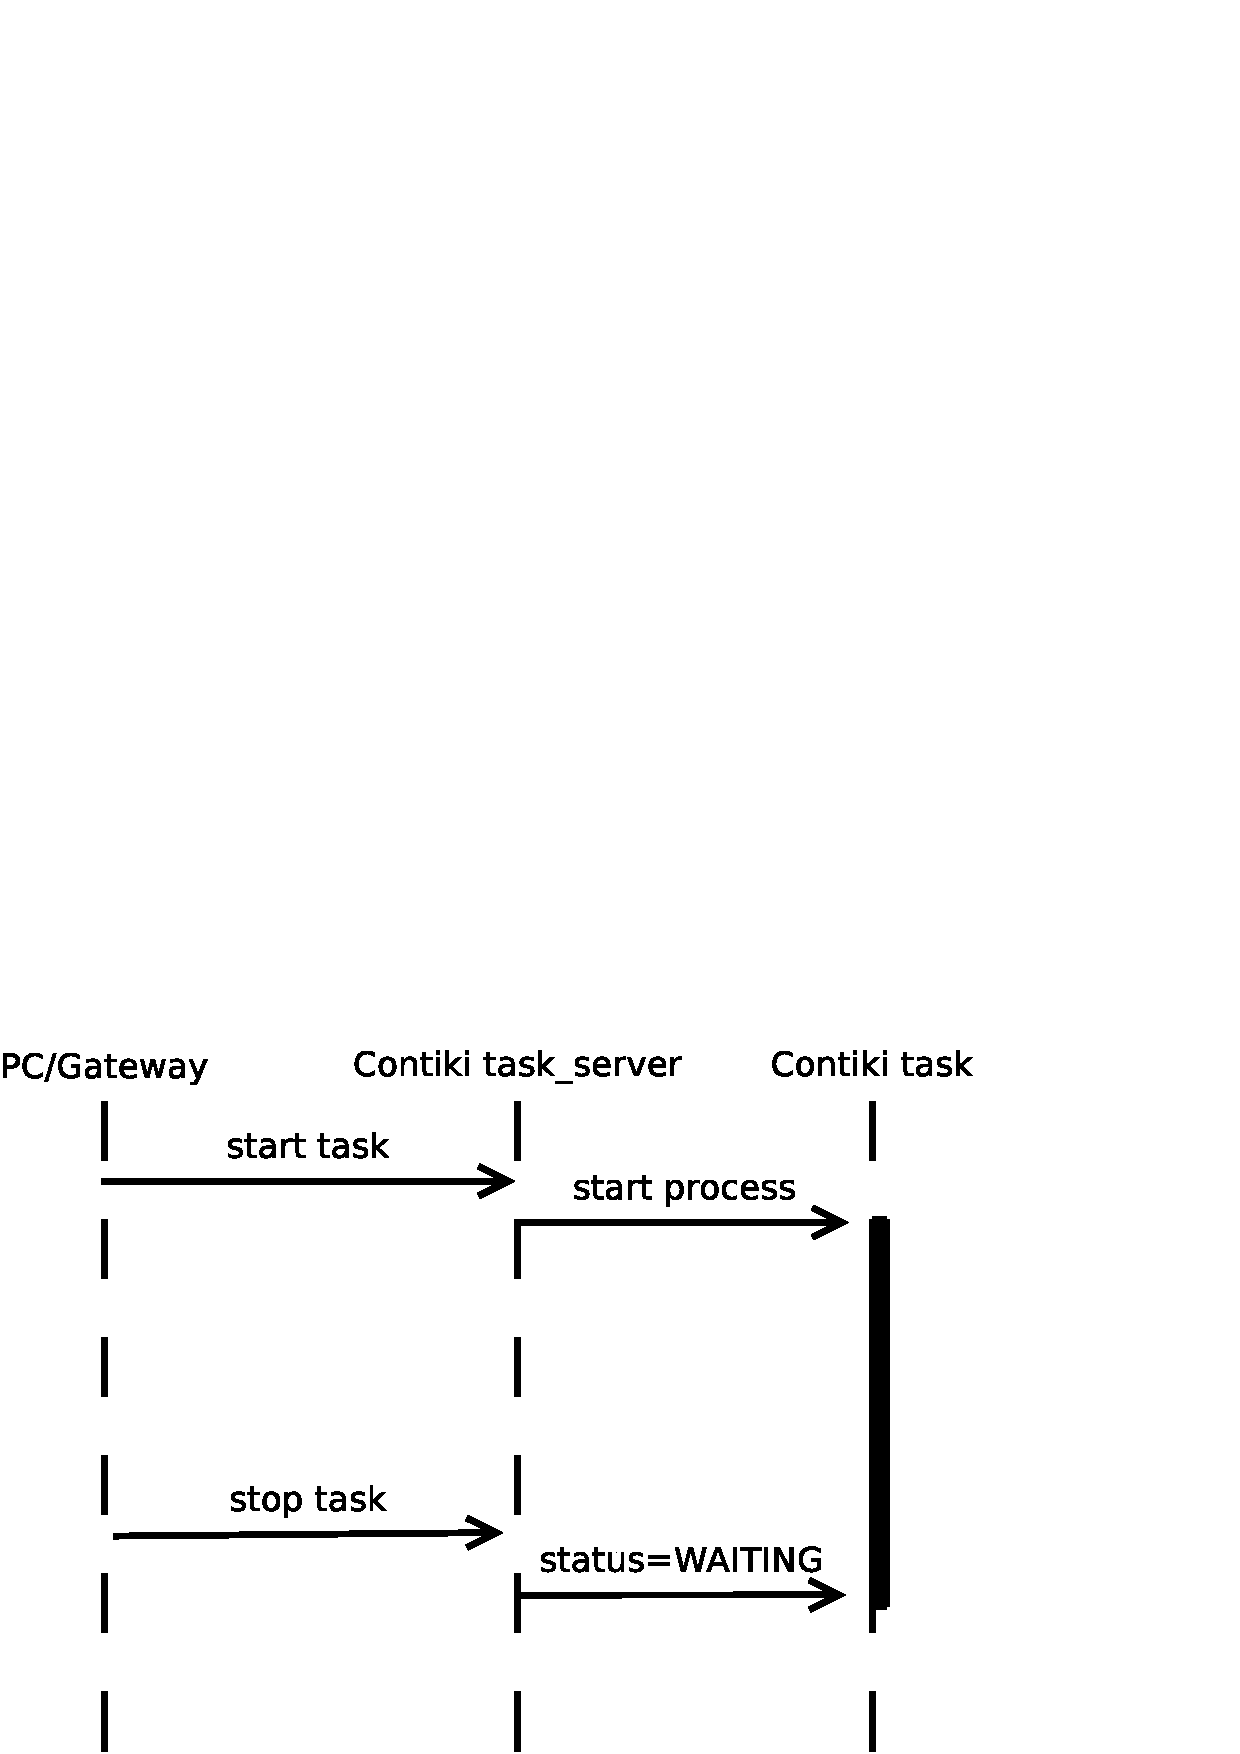
\includegraphics[scale=0.5]{img/starttask.pdf}
	\end{center}
	\caption{\small \itshape{The exchange of messages while starting/stopping tasks}}
\end{figure}

\lstset{numbers=left, mathescape=true, nolol=false,caption=Task server snippet,label=lst:taskserver}
\begin{lstlisting}
PROCESS_THREAD(task_server_process, ev, data)
{
	PROCESS_BEGIN();

	list_init(task_list);

	list_add(task_list,&el_monitor_process);
	list_add(task_list,&el_delay_process);
	list_add(task_list,&el_temperature_sensing);

	tcp_listen(HTONS(1010));

	while(1) 
	{
		PROCESS_WAIT_EVENT_UNTIL(ev == tcpip_event);

		if(uip_connected()) 
		{
			PSOCK_INIT(&ps, buffer, sizeof(buffer));

			while(!(uip_aborted() || uip_closed() 
			|| uip_timedout())) 
			{
				PROCESS_WAIT_EVENT_UNTIL
				(ev == tcpip_event);
				handle_connection(&ps);
			}
		}
	}
	PROCESS_END();
}
\end{lstlisting}

% ********** End of Software platform **********
